% Названия под-под-разделов указываем в стиле:
% \subsubsect{метка для ref}
%   {отображаемое название под-под-раздела}

В данном разделе мы приводим рекомендации и примеры оформления различных типовых элементов отчета: формул (см. раздел~\ref{sec:demo_examples_formulas}), рисунков (см. раздел~\ref{sec:demo_examples_figures}), таблиц (см. раздел~\ref{sec:demo_examples_tables}), различных вспомогательных команд (см. раздел~\ref{sec:demo_examples_commands}) и иных элементов (см. раздел~\ref{sec:demo_examples_various}).

\subsubsect{sec:demo_examples_formulas}
  {Оформление формул}

  Формулы оформляются стандартным образом.
  Отметим, что все формулы (даже те, на которые нет ссылок в тексте) стоит нумеровать.
  Перед формулой ставится двоеточие, а после формулы необходимо вставить знак препинания (запятая или точка).

  Для произвольного элемента $(i_1,\ldots,i_d)$ тензора $\tens{A} \in \set{R}^{N_1 \times N_2 \times \ldots \times N_d}$, разложение тензорного поезда (TT-разложение) может быть записано как:
  \begin{equation}\label{eq:decomp_tt}
    \begin{split}
      \tens{Y} [n_1, n_2, \ldots, n_d] =
        \sum_{r_1=1}^{R_1}
        \sum_{r_2=1}^{R_2}
        \cdots
        \sum_{r_{d-1}=1}^{R_{d-1}}
          &
          \tens{G}_1 [1, n_1, r_1]
          \tens{G}_2 [r_1, n_2, r_2]
          \cdots \times
          \\
          \times
          &
          \tens{G}_{d-1} [r_{d-2}, n_{d-1}, r_{d-1}]
          \tens{G}_d [r_{d-1}, n_d, 1],
    \end{split}
  \end{equation}
  где числа $(R_1, R_2, \ldots, R_d)$ --- это TT-ранги (обычно для упрощения записи формально вводятся также ранги $R_0=R_d=1$), а трехмерные тензоры $\tens{G}_1, \tens{G}_2, \ldots, \tens{G}_d$ --- ядра TT-разложения ($\tens{G}_1$ и $\tens{G}_d$ являются двухмерными тензорами, но формально могут рассматриваться как трехмерные тензоры с единичным размером первой и последней моды соответственно).
  TT-разложение~\eqref{eq:decomp_tt} также может быть записано в более компактной матричной форме:
  \begin{equation}
  	\tens{A}[i_1, i_2, \ldots, i_d]
  	=
  	\matr{G}_1(i_1)
  	\matr{G}_2(i_2)
  	\ldots
  	\matr{G}_d(i_d).
  \end{equation}
  В последней формуле $\matr{G}_k(i_k)$ --- это ядра TT-разложения, записанные в виде матриц размера $R_{k-1} \times R_k$.

\subsubsect{sec:demo_examples_figures}
  {Оформление рисунков}

  \begin{figure}[!t]
    \centering
    
\includegraphics[width=0.5\linewidth]{tensor_train.png}
    \caption{
      Схематическая форма представления разложения тензорного поезда
    }
    \label{fig:tensor_train}
  \end{figure}

  \begin{figure}[t!]
    \centering
    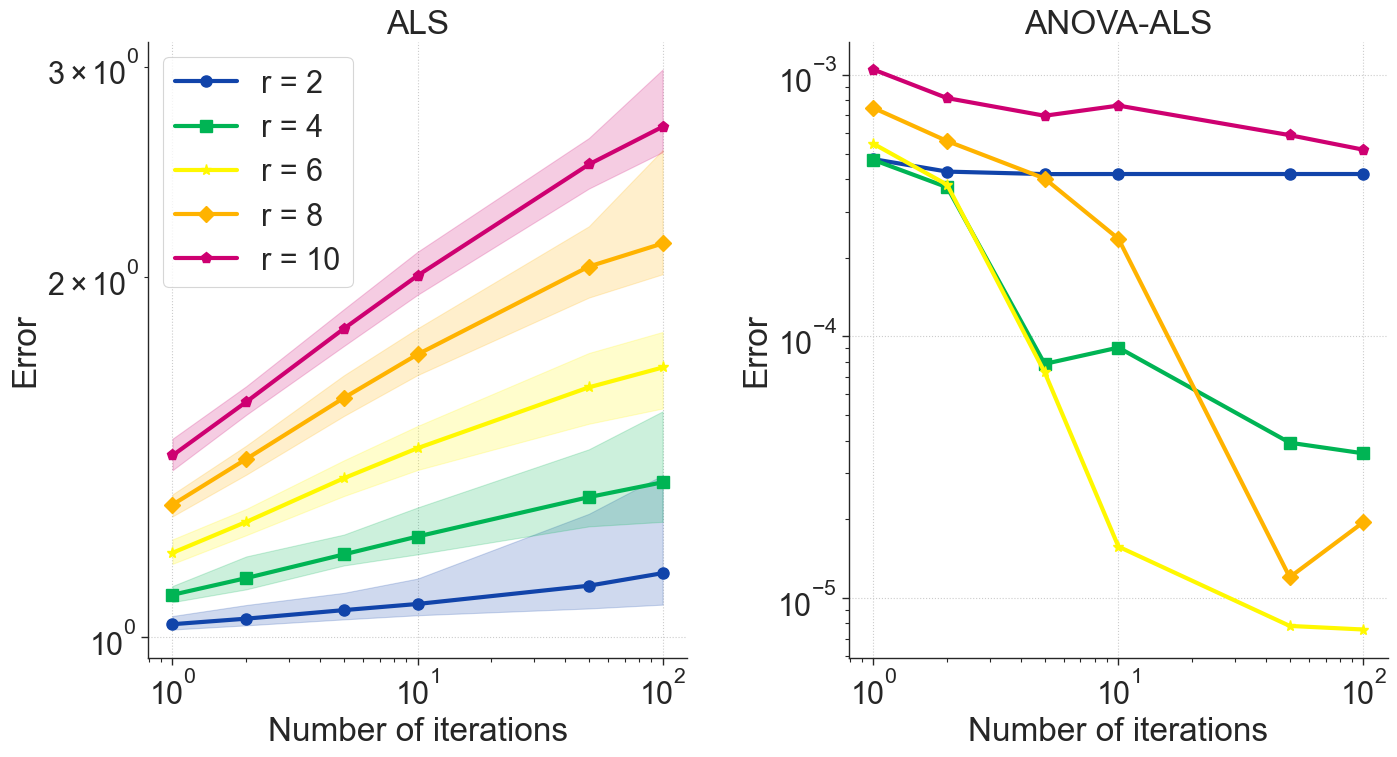
\includegraphics[scale=0.4]{something.png}
    \caption{
      Ошибка приближения целевой величины стандартным методом \func{TT-ALS} (на графике слева) и предлагаемым методом \func{TT-ANOVA-ALS} (на графике справа)
    }
    \label{fig:demo_two_pict}
  \end{figure}

  \begin{figure}[t]
    \begin{minipage}{.37\textwidth}
      \centering
      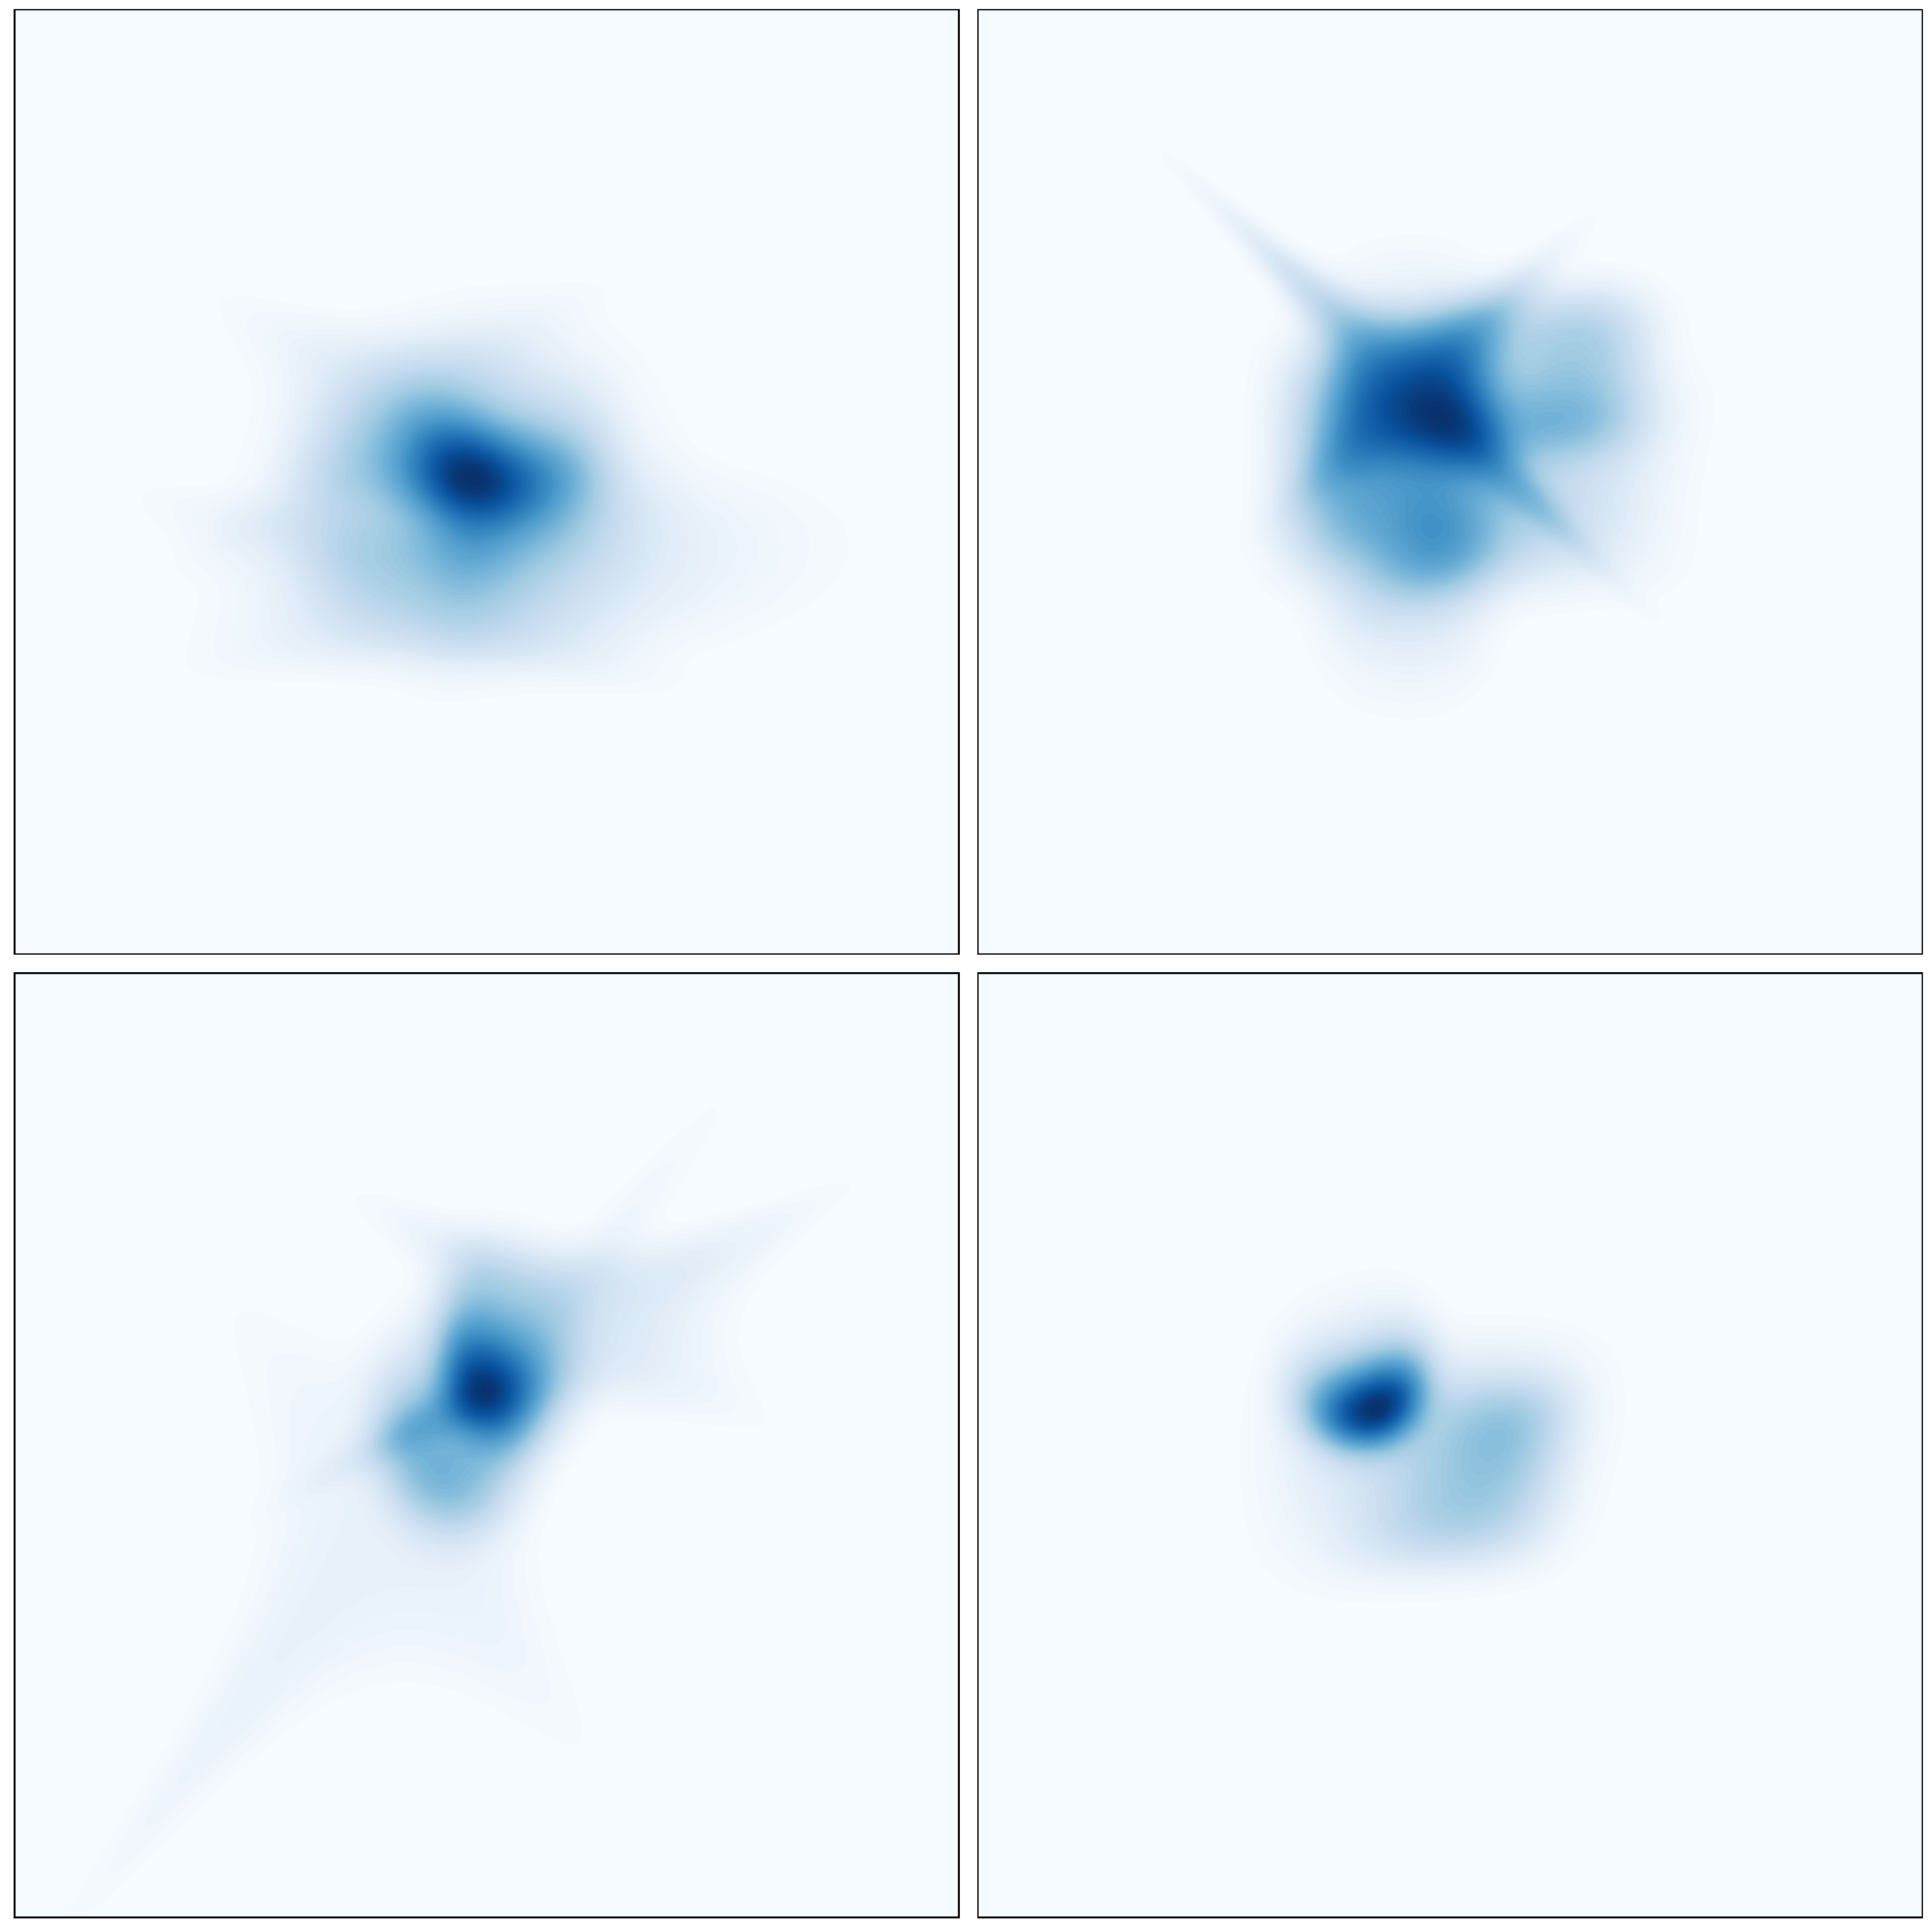
\includegraphics[width=0.99\linewidth]{mixtures.pdf}
      \captionof{figure}{
        Пример двумерного распределения, соответствующего какой-то ерунде
      }
      \label{fig:mixtures_example}
    \end{minipage}
    \hspace{.03\textwidth}
    \begin{minipage}{.57\textwidth}
      \centering
      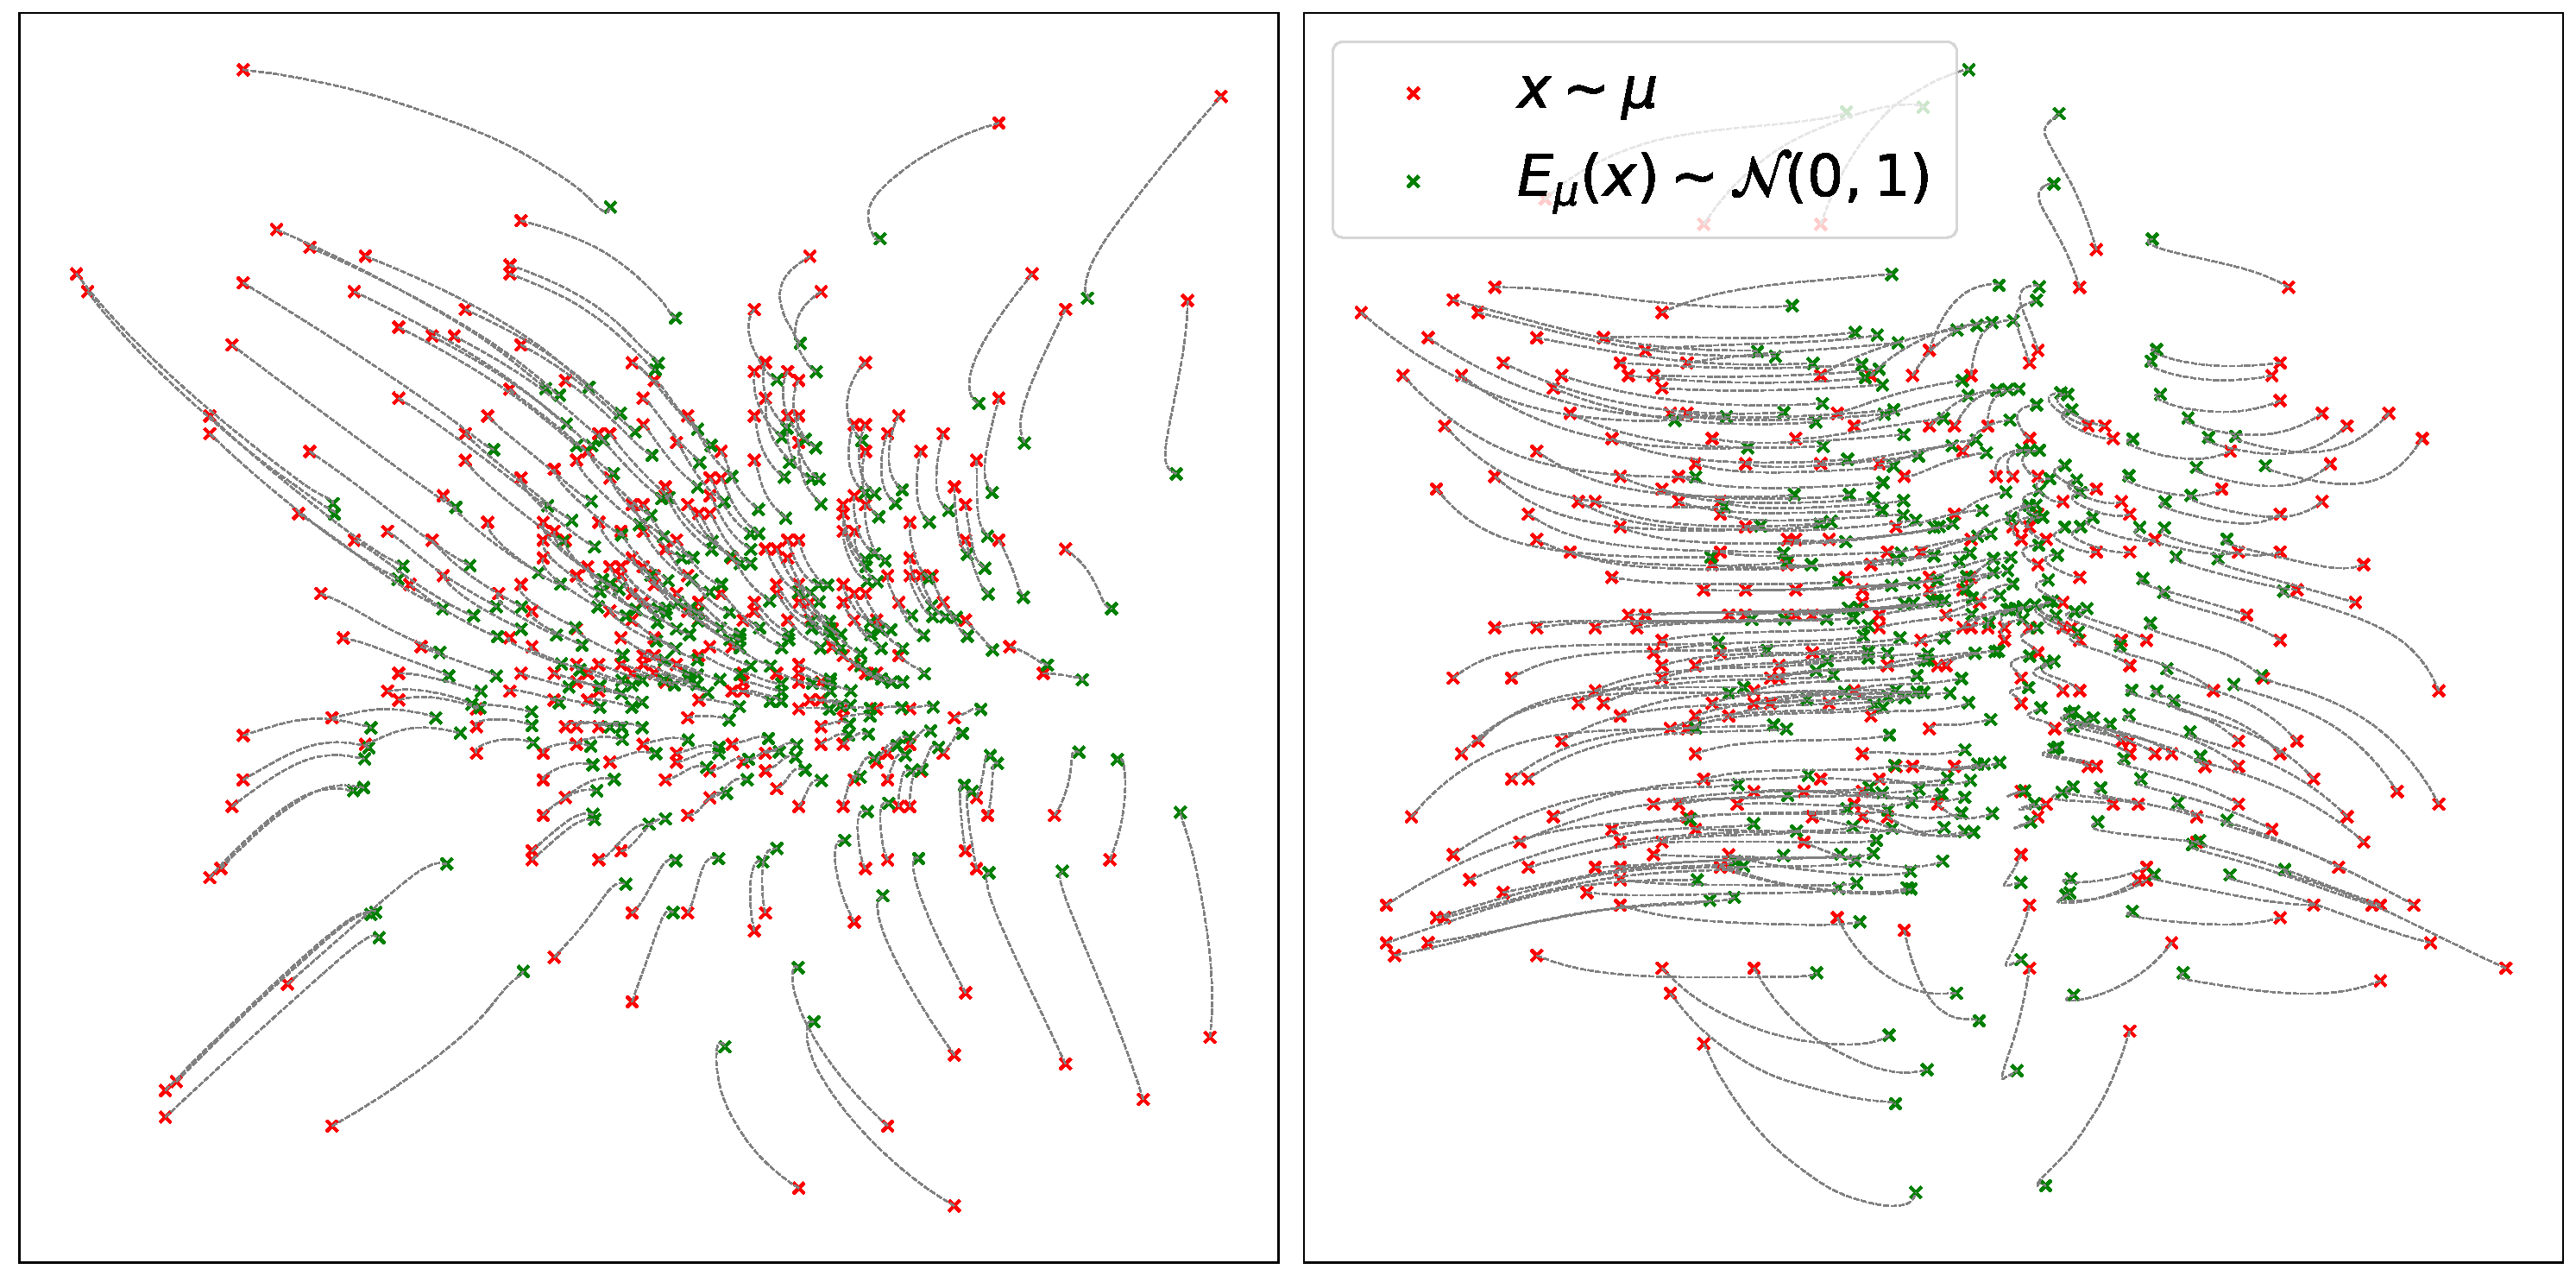
\includegraphics[width=0.99\linewidth]{nonlinear.pdf}
      \vskip 0.155in
      \captionof{figure}{
        Пример траекторий каких-то там потоков, текущих куда-то
      }
      \label{fig:plot_example_nonlinear}
    \end{minipage}
  \end{figure}

  На рисунке~\ref{fig:tensor_train} в схематической форме приводится общий вид TT-разложения.
  Можно делать подпись сразу к двум картинкам как показано на рисунке~\ref{fig:demo_two_pict}.
  Если <<очень приспичит>>, то можно и вот так оформлять рисунки: на рисунке~\ref{fig:mixtures_example} изображена одна фигня, а на рисунке~\ref{fig:plot_example_nonlinear} -- другая фигня.

  Файлы с графическими изображениями должны храниться в папке <<images>>.
  Рисунки удобно размещать в верхней части листов, <<разбавляя>> пространство между последовательными рисунками текстом.
  Отметим, что в конце подписи к рисунку точка не ставится.

\subsubsect{sec:demo_examples_tables}
  {Оформление таблиц}

  \begin{table}[t!]
    \caption{
      Модельные функции из работы~\cite{chertkov2022black} для анализа методов аппроксимации
    }
    \label{tbl:demo}
    \centering
    \begin{small}
    \renewcommand{\arraystretch}{2.5}
    \begin{tabular}{|p{3.0cm}|p{2.0cm}|p{1.6cm}|p{8.5cm}|}\hline
      Функция                &
      Ссылка                 &
      Область                &
      Аналитическая формула
      \\ \hline

      \func{Rosenbrock}
          & \cite{jamil2013literature}
          & [$-2.048$, $2.048$]
          &
          $
          \func{f}(\vect{x})
          =
          \sum_{i=1}^{d-1} \left(
              100 \cdot (x_{i+1} - x_{i}^2)^2 + (1 - x_{i})^2
          \right)
          $
          \\ \hline

      \func{Schaffer}
          & \cite{jamil2013literature}
          & [$-100$, $100$]
          &
          $
          \func{f}(\vect{x})
          =
          \sum_{i=1}^{d-1} (
              0.5 +
              \frac{
                  \sin^2{\left( \sqrt{x_i^2 + x_{i+1}^2} \right)} - 0.5
              }{
                  \left( 1 + 0.001 (x_i^2 + x_{i+1}^2)\right)^2
              }
          )
          $
          \\ \hline

      \func{Schwefel}
          & \cite{dieterich2012empirical}
          & [$-500$, $500$]
          &
          $
          \func{f}(\vect{x})
          =
          418.9829 \cdot d - \sum_{i=1}^d x_i \cdot \sin{(\sqrt{|x_i|})}
          $
          \\ \hline

    \end{tabular}
    \end{small}
  \end{table}

  Таблицы оформляются стандартным образом.
  В качестве примера см. таблицу~\ref{tbl:demo}.
  Отметим, что в конце подписи к таблице точка не ставится.

\subsubsect{sec:demo_examples_commands}
  {Вспомогательные команды}

  В файле <<commands.tex>> приводятся различные удобные вспомогательные команды для отображения различных математических объектов и операций, в том числе:
  \begin{enumerate}
    \item Жирный шрифт
      \fat{в тексте} или в формуле $x^2 = \fat{y^4}$;
    \item Множество
      $\in \set{N}$ или $\in \set{R}$;
    \item Вектор
      $\vect{x} \in \set{R}^{N_1}$;
    \item Матрица
      $\matr{X} \in \set{R}^{N_1 \times N_2}$;
    \item Тензор
      $\tens{X} \in \set{R}^{N_1 \times N_2 \times \ldots \times N_d}$;
    \item Функция
      $\func{f}(\vect{x})$;
    \item Вектор-функция
      $\vfunc{f}(\vect{x})$;
    \item Функционал
      $\ffunc{f}(\poi)$;
    \item Оператор
      $\oper{W}$;
    \item След матрицы
      $\trace{\matr{A}}$;
    \item Порядок
      $\order{n^2}$;
    \item Дивергенция
      $\divergence{\vect{x}}$;
    \item Производная
      $\der{f}{x}$;
    \item Производная по времени
      $\dert{f}$;
    \item Производная по $x$
      $\derx{f}$;
    \item Частная производная
      $\pder{f}{z}$;
    \item Частная производная по времени
      $\pdert{f}$;
    \item Частная производная по $x$
      $\pderx{f}$;
    \item Частная производная по компоненте координаты
      $\pderxi{f}{3}$;
    \item Векторизация
      $\vectorize{\tens{X}}$;
    \item Построение вектора
      $\vectl{1, 2, \ldots, d}$;
    \item Построение индекса из мульти-индекса
      $i = \iflatten{i_1, i_2, \ldots, i_d}$;
    \item Построение мульти-индекса из индекса
      $\vect{i} = \imulti{i}$;
    \item Точка
      $\ffunc{f}(\poi)$;
    \item Заметка \note{Надо будет все уточнить}.
  \end{enumerate}

\subsubsect{sec:demo_examples_various}
  {Разное}

  Можно и нужно использовать сноски для вспомогательных комментариев, например, для пояснения, что такое тензор\footnote{
    Здесь и далее (в соответствии с нормами современной вычислительной математики и машинного обучения) термин \textit{тензор} является фактически синонимом для термина \textit{многомерный массив}.
    } и~т.п.
  Ссылки на статьи оформляются стандартным образом, см., например, работу~\cite{oseledets2011tensortrain} или работы~\cite{dieterich2012empirical, jamil2013literature, singh2019abstract}.
  \note{На данный момент русскоязычные записи в библиографии часто приводят к ошибкам, будет исправлено.}

  Отметим, что малоранговая аппроксимация на основе TT-разложения~\cite{oseledets2011tensortrain} представляет один из распространенных подходов для компактного приближения функций многих переменных, включая приложения в области анализа данных и машинного обучения.
  В работе~\cite{oseledets2011tensortrain} доказывается теорема существования точного TT-представления с рангами~$R_k$ не выше, чем $rank \, \matr{A}^{\langle k \rangle}$, где $\matr{A}^{\langle k \rangle}$ --- это $k$-ая матричная развертка тензора.
